\apendice{Documentación de usuario}

\section{Requisitos software y hardware para ejecutar el proyecto.}

En esta sección del anexo se definen varios requisitos tanto de software como de hardware que requiere el dispositivo objeto de este trabajo. Cuantos más requisitos cumpla el prototipo más exitoso resultará el dispositivo. 

\subsection{Requisitos funcionales}

%%%%%%%%%%%%%%%%%%%%%%%%%%%%% RF-01 %%%%%%%%%%%%%%%%%%%%%%%%%%%%
\begin{table}[h!]
\begin{tabular}{|
>{\columncolor[HTML]{EFEFEF}}c |l|}
\hline
\cellcolor[HTML]{B9E3F0}\textbf{RF-01} & \multicolumn{1}{c|}{\cellcolor[HTML]{B9E3F0}\textbf{Aplicación}}                                                                                                                                                                                \\ \hline
Descripción                            & \begin{tabular}{p{10.5cm}}La solución deberá contar con una aplicación, ya sea una aplicación de escritorio, web o móvil, para simplificar la experiencia de uso y la visualización de resultados por parte del usuario.\end{tabular} \\ \hline
Importancia                            & \cellcolor[HTML]{FFFFFF}\begin{tabular}{p{10.5cm}}Alta, es la base de la visualización del seguimiento de la persona que utiliza el dispositivo.\end{tabular}                                                                               \\ \hline
Prioridad                              & \multicolumn{1}{c|}{Alta}                                                                                                                                                                                                                       \\ \hline
\end{tabular}
\caption{Requisito Funcional 1 'Aplicación'}
\label{RF_01}
\end{table}

%%%%%%%%%%%%%%%%%%%%%%%%%%%%% RF-02 %%%%%%%%%%%%%%%%%%%%%%%%%%%%
\begin{table}[h!]
\begin{tabular}{|
>{\columncolor[HTML]{EFEFEF}}c |l|}
\hline
\cellcolor[HTML]{B9E3F0}\textbf{RF-02} & \multicolumn{1}{c|}{\cellcolor[HTML]{B9E3F0}\textbf{Iniciar grabación}}                                                                                                                                                                                \\ \hline
Descripción                            & \begin{tabular}{p{10.5cm}}La solución deberá contar con una opción de grabación, con la cual el profesional o el usuario tendrán la posibilidad de comenzar y finalizar el registro de la postura.\\ Los resultados durante la grabación se almacenarán en la plataforma para su análisis.\end{tabular} \\ \hline
Importancia                            & \cellcolor[HTML]{FFFFFF}\begin{tabular}{p{10.5cm}}Alta, ya que la grabación de las respuestas permitirá al profesional analizarlas de forma detallada con el objetivo de obtener conclusiones y determinar el grado y evolución de la afectación.\end{tabular}                                                                               \\ \hline
Prioridad                              & \multicolumn{1}{c|}{Alta}                                                                                                                                                                                                                       \\ \hline
\end{tabular}
\caption{Requisito Funcional 2 'Iniciar grabación'}
\label{RF_02}
\end{table}

%%%%%%%%%%%%%%%%%%%%%%%%%%%%% RF-03 %%%%%%%%%%%%%%%%%%%%%%%%%%%%
\begin{table}[h!]
\begin{tabular}{|
>{\columncolor[HTML]{EFEFEF}}c |l|}
\hline
\cellcolor[HTML]{B9E3F0}\textbf{RF-03} & \multicolumn{1}{c|}{\cellcolor[HTML]{B9E3F0}\textbf{Identificación de perfiles}}                                                                                                                                                                                \\ \hline
Descripción                            & \begin{tabular}{p{10.5cm}}La aplicación debe ser capaz de diferenciar a diferentes perfiles, en el caso de uso de una organización o un profesional, y una única identificación en el caso de que se trate de un usuario particular.\end{tabular} \\ \hline
Importancia                            & \cellcolor[HTML]{FFFFFF}\begin{tabular}{p{10.5cm}}Media, una vez se obtenga la base del dispositivo y su funcionamiento se puede dividir a los usuarios entre profesionales o particulares, con distintas funciones para cada uno de ellos.\end{tabular}                                                                               \\ \hline
Prioridad                              & \multicolumn{1}{c|}{Media}                                                                                                                                                                                                                       \\ \hline
\end{tabular}
\caption{Requisito Funcional 3 'Identificación de perfiles'}
\label{RF_03}
\end{table}

%%%%%%%%%%%%%%%%%%%%%%%%%%%%% RF-04 %%%%%%%%%%%%%%%%%%%%%%%%%%%%
\begin{table}[h!]
\begin{tabular}{|
>{\columncolor[HTML]{EFEFEF}}c |l|}
\hline
\cellcolor[HTML]{B9E3F0}\textbf{RF-04} & \multicolumn{1}{c|}{\cellcolor[HTML]{B9E3F0}\textbf{Detección de la postura}}                                                                                                                                                                                \\ \hline
Descripción                            & \begin{tabular}{p{10.5cm}}La solución deberá ser capaz de detectar los cambios en la postura. Para ello, se deberá implementar un algoritmo que filtre en función de los datos en crudo recogidos, una postura correcta o incorrecta. Esta medición se podría obtener en forma de ‘porcentaje de buena postura’.\end{tabular} \\ \hline
Importancia                            & \cellcolor[HTML]{FFFFFF}\begin{tabular}{p{10.5cm}}Alta, dado que es la base que permitirá definir si la persona lleva una buena postura o no, y en base a ello, realizar la comunicación correspondiente y obtener las estadísticas necesarias para la toma de decisiones.\end{tabular}                                                                               \\ \hline
Prioridad                              & \multicolumn{1}{c|}{Alta}                                                                                                                                                                                                                       \\ \hline
\end{tabular}
\caption{Requisito Funcional 4 'Detección postural'}
\label{RF_04}
\end{table}

%%%%%%%%%%%%%%%%%%%%%%%%%%%%% RF-05 %%%%%%%%%%%%%%%%%%%%%%%%%%%%
\begin{table}[h!]
\begin{tabular}{|
>{\columncolor[HTML]{EFEFEF}}c |l|}
\hline
\cellcolor[HTML]{B9E3F0}\textbf{RF-05} & \multicolumn{1}{c|}{\cellcolor[HTML]{B9E3F0}\textbf{Comunicar una postura incorrecta}}                                                                                                                                                                                \\ \hline
Descripción                            & \begin{tabular}{p{10.5cm}}La solución debe poder comunicar mediante, vibración, sonido u otra manera una mala postura continuada durante un periodo de tiempo predefinido.\end{tabular} \\ \hline
Importancia                            & \cellcolor[HTML]{FFFFFF}\begin{tabular}{p{10.5cm}}Alta, es necesario que el usuario conozca en todo momento su situación, para poder corregir su postura cuando sea necesario.\end{tabular}                                                                               \\ \hline
Prioridad                              & \multicolumn{1}{c|}{Media}                                                                                                                                                                                                                       \\ \hline
\end{tabular}
\caption{Requisito Funcional 5 'Comunicar una postura incorrecta'}
\label{RF_05}
\end{table}

%%%%%%%%%%%%%%%%%%%%%%%%%%%%% RF-06 %%%%%%%%%%%%%%%%%%%%%%%%%%%%
\begin{table}[h!]
\begin{tabular}{|
>{\columncolor[HTML]{EFEFEF}}c |l|}
\hline
\cellcolor[HTML]{B9E3F0}\textbf{RF-06} & \multicolumn{1}{c|}{\cellcolor[HTML]{B9E3F0}\textbf{Realizar seguimiento}}                                                                                                                                                                                \\ \hline
Descripción                            & \begin{tabular}{p{10.5cm}}La información registrada por el dispositivo debe quedar almacenada para valorar y evaluar la postura del paciente, con el fin de modificar o no el tratamiento o fisioterapia o tomar otro tipo de decisiones.\\ La visualización de la información recogida se reflejará en forma de gráficos y tablas. Esto permitirá analizar la información de manera clara y sencilla
\end{tabular} \\ \hline
Importancia                            & \cellcolor[HTML]{FFFFFF}\begin{tabular}{p{10.5cm}}Alta, ya que será clave para la toma de decisiones por parte del especialista en cuanto a la personalización del tratamiento y rehabilitación.\end{tabular}                                                                               \\ \hline
Prioridad                              & \multicolumn{1}{c|}{Alta}                                                                                                                                                                                                                       \\ \hline
\end{tabular}
\caption{Requisito Funcional 6 'Realizar seguimiento'}
\label{RF_06}
\end{table}

%%%%%%%%%%%%%%%%%%%%%%%%%%%%% RF-07 %%%%%%%%%%%%%%%%%%%%%%%%%%%%
\begin{table}[h!]
\begin{tabular}{|
>{\columncolor[HTML]{EFEFEF}}c |l|}
\hline
\cellcolor[HTML]{B9E3F0}\textbf{RF-07} & \multicolumn{1}{c|}{\cellcolor[HTML]{B9E3F0}\textbf{Manual de usuario}}                                                                                                                                                                                \\ \hline
Descripción                            & \begin{tabular}{p{10.5cm}}La solución deberá incluir unas instrucciones que se entreguen al usuario que lo vaya a utilizar. Esto supone un apoyo durante todo el proceso de uso del dispositivo y de la aplicación por parte del usuario.\end{tabular} \\ \hline
Importancia                            & \cellcolor[HTML]{FFFFFF}\begin{tabular}{p{10.5cm}}Media, puesto que supone un apoyo para el usuario que lo utilice.\end{tabular}                                                                               \\ \hline
Prioridad                              & \multicolumn{1}{c|}{Baja}                                                                                                                                                                                                                       \\ \hline
\end{tabular}
\caption{Requisito Funcional 7 'Manual de usuario'}
\label{RF_07}
\end{table}

\clearpage
%%%%%%%%%%%%%%%%%%%%%%%%%%%%% RF-08 %%%%%%%%%%%%%%%%%%%%%%%%%%%%
\begin{table}[]
\begin{tabular}{|
>{\columncolor[HTML]{EFEFEF}}c |l|}
\hline
\cellcolor[HTML]{B9E3F0}\textbf{RF-08} & \multicolumn{1}{c|}{\cellcolor[HTML]{B9E3F0}\textbf{Batería}}                                                                                                                                                                                \\ \hline
Descripción                            & \begin{tabular}{p{10.5cm}}El dispositivo debe disponer de una batería para poder utilizarlo de forma telemática. Además, la batería del dispositivo debe ser suficiente para el uso previsto.\end{tabular} \\ \hline
Importancia                            & \cellcolor[HTML]{FFFFFF}\begin{tabular}{p{10.5cm}}Media, se debe incluir para mayor comodidad y libertad del paciente al utilizar el dispositivo.\end{tabular}                                                                               \\ \hline
Prioridad                              & \multicolumn{1}{c|}{Media}                                                                                                                                                                                                                       \\ \hline
\end{tabular}
\caption{Requisito Funcional 8 'Batería'}
\label{RF_08}
\end{table}

%\clearpage

\subsection{Requisitos no funcionales}
\begin{itemize}
    \item \textbf{Accesibilidad}: la aplicación debe ser accesible para el mayor grupo de personas posible, tengan o no algún tipo de discapacidad.
    \item \textbf{Seguridad}: el dispositivo electrónico debe ser seguro y la información manejada en la aplicación debe estar protegida.
    \item \textbf{Compatibilidad}: la aplicación debe ser compatible con distintos dispositivos.
    \item \textbf{Eficiencia}: la aplicación debe permitir al usuario lograr sus objetivos, con un coste computacional y temporal bajo.
    \item \textbf{Efectividad}: la aplicación debe cumplir con exactitud los requisitos funcionales. 
    \item \textbf{Errores}: la aplicación debe presentar una tasa de error baja, además, debe mostrar posibles soluciones en caso de anomalías.
    \item \textbf{Usabilidad}: tanto el uso del dispositivo electrónico como de la aplicación debe ser sencillo, es decir, se debe poder usar de forma intuitiva.
    \item \textbf{Memorabilidad}: tanto el funcionamiento del dispositivo electrónico como de la aplicación debe ser fácil de recordar, tras no haberlos utilizado durante un tiempo.
    \item \textbf{Satisfacción}: el usuario debe estar satisfecho con el dispositivo electrónico y la aplicación, tanto por su comodidad, estética y usabilidad.


\end{itemize}

%%%%%%%%%%%%%%%%%%%%%%%%%%%%%%%%%%%%%%
\clearpage
% Otra opción para salto de página \newpage
\section{Instalación / Puesta en marcha}
Como se han creado dos versiones los requisitos de instalación y puesta en marcha serán diferentes.

Para la primera versión del prototipo dónde se emplea el sensor SW520D\cite{SW520D_1}, es necesario tener instalado el software de Arduino IDE\cite{ArduinoIDE,Arduino1,Arduino2}, sin necesidad de instalar cualquier librería adicional.

Mientras que para la segunda versión no solo se ha de tener instalado el software de Arduino IDE, sino que se deberá igualmente tener instaladas las librerías I2Cdev\cite{LibI2Cdev}, MPU6050\cite{LibMPU6050} y Wire\cite{LibWire}: 

Una vez tenemos instalado el software y las librerías necesarias, el siguiente paso será el de montar el prototipo siguiendo los esquemas especificados en las figuras \textit{Figura \ref{fig:ProtV1}} y \textit{Figura \ref{fig:ProtV2}}.

\textcolor{red}{Incluir El repositorio de GitHub}

Si se ha montado la primera versión del prototipo se deberá descargar el programa que se encuentra en el repositorio de GitHub\cite{GitHub} bajo el nombre de 'PrototipoV1.ino'. En el caso de haber montado la segunda versión, se deberá descargar el programa del repositorio de GitHub\cite{GitHub} con el nombre de 'PrototipoV2.ino'. Estos programas son los que abriremos y se enviarán al microprocesador Arduino UNO R3\cite{Arduino2}, el prototipo montado, que se encontrará conectado con el cable USB al ordenador. Una vez cargados los programas se podrá realizar el control postural, de forma que se consiga una ejecución exitosa.


\subsection{Versión 1, empleando el sensor SW520D}
Como primera versión se ha creado un prototipo empleando Arduino\cite{Arduino1} y el sensor SW520D\cite{SW520D_1}.

Se ha incluido un botón de encendido, un led de color azul que indica que el dispositivo se encuentra encendido, un zumbador pasivo que actuará como señal sonora y un motor de vibración que actuará como aviso vibratorio.

Cuando el sensor detecta que la persona se ha inclinado hacia delante, se detecta una mala postura y salta una alerta sonora (melodía modificable empleando el zumbador) y vibratoria (motor de vibración).

Se pueden observar los componentes y las conexiones realizadas en esta versión en los diagramas \textit{Figura \ref{fig:ProtV1}} y \textit{Figura \ref{fig:ProtV1_esquema}}. 

\begin{figure}[h!]
    \centering
    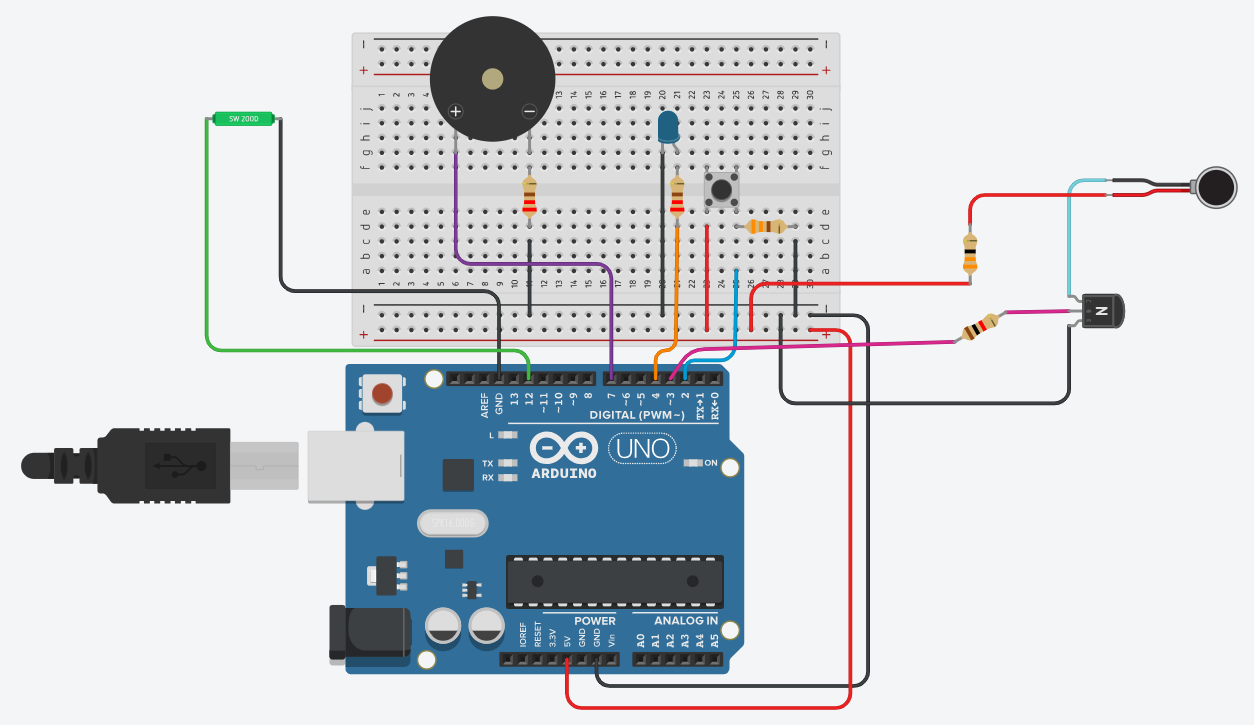
\includegraphics[width=0.8\textwidth]{img/PrototipoV1_Tilt.png}
    \caption{Diagrama de la primera versión del prototipo, empleando el sensor SW520D}
    \label{fig:ProtV1}
\end{figure}

\begin{figure}[h]
    \centering
    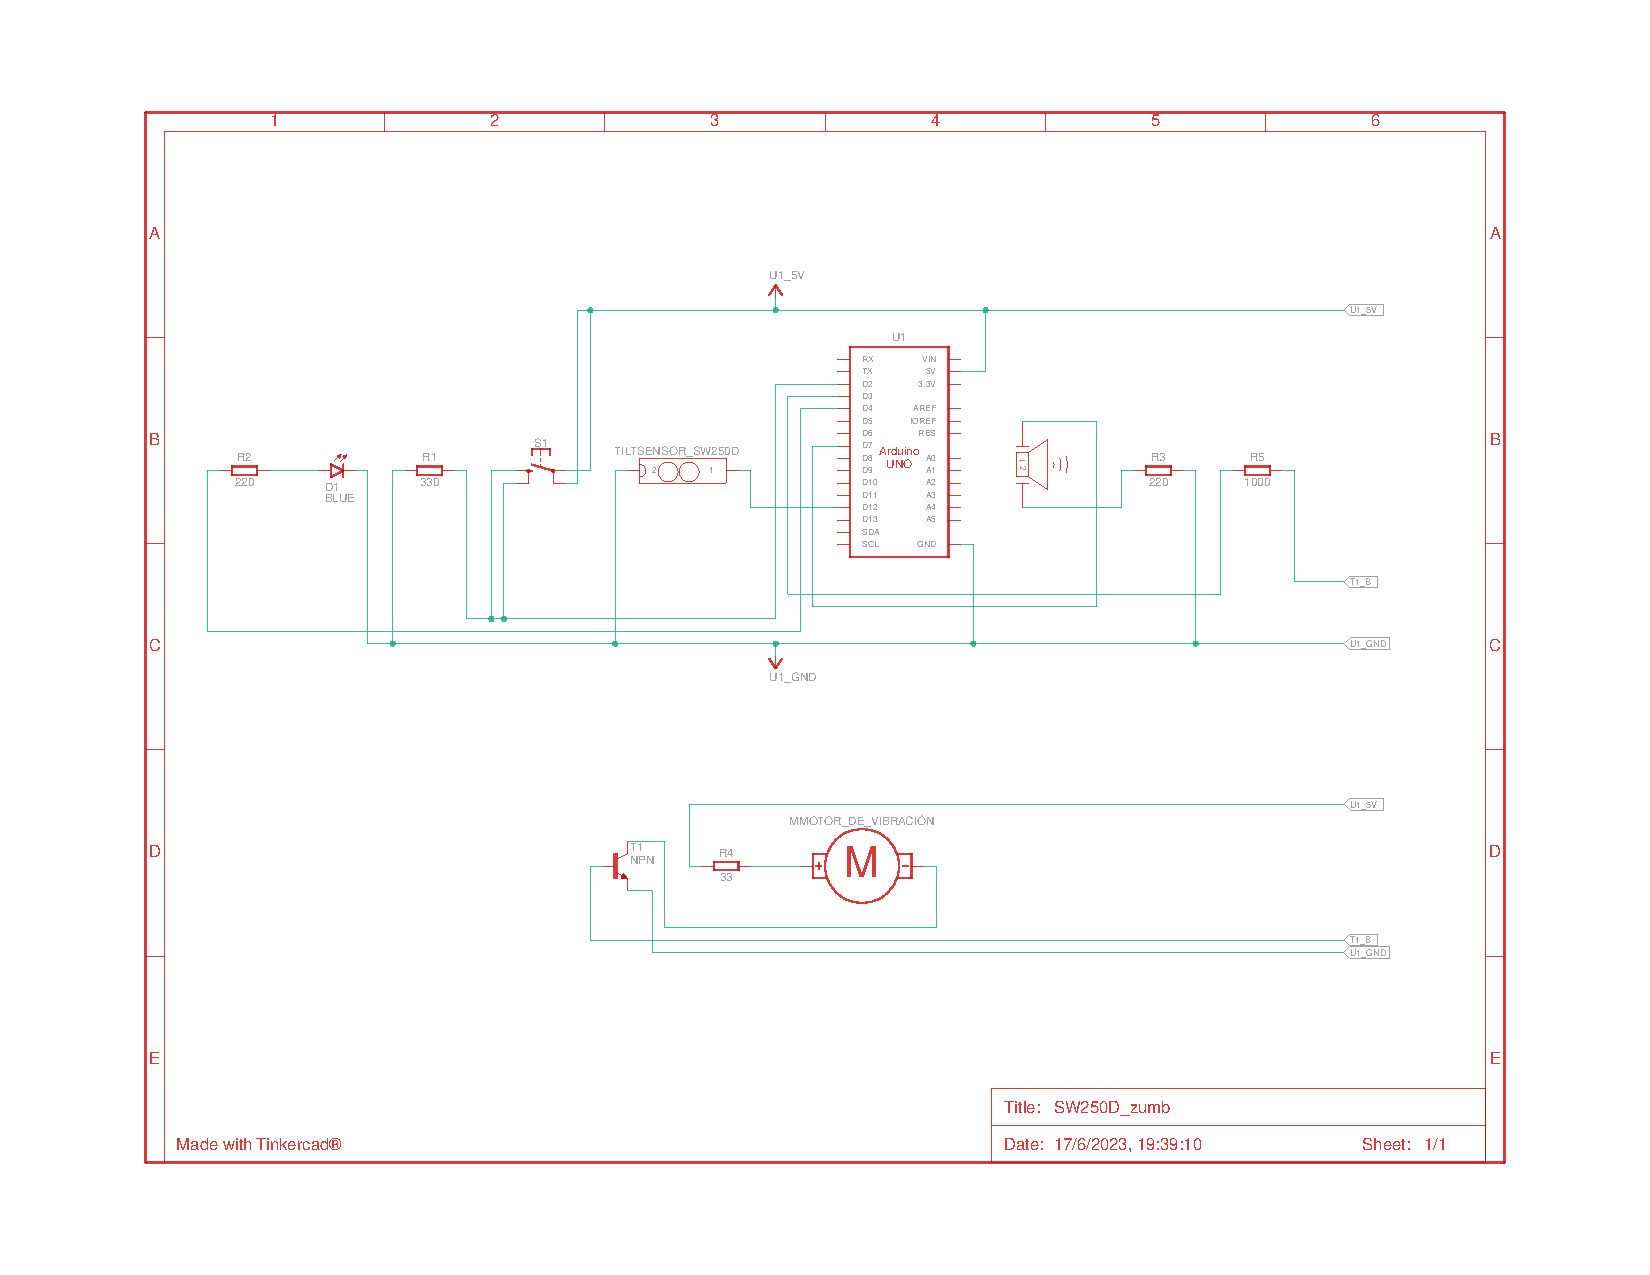
\includegraphics[width=0.9\textwidth]{img/Prot_V1_Esquema.pdf}
    \caption{Diagrama de las realizadas para la implementación de la primera versión del prototipo.}
    \label{fig:ProtV1_esquema} 
\end{figure}


\newpage
El código empleado para el funcionamiento de esta primera versión ha sido el siguiente:
\begin{lstlisting}
// Led simple + Boton + Zumbador + Tilt + Motor Vibracion
// Naiara Gadea Rodriguez Gomez
// 

int led = 4; // Seleccion del pin del led (pin digital)
int  boton = 2; // Seleccion del pin del boton (pin digital)
int zum = 7;// Seleccion del pin del zumbador
int tilt = 12;// Seleccion del pin del sensor SW250D
int motor = 3; //Seleccion del pin del motor de vibracion

int estado; // Estado del boton

void setup() {
  Serial.begin(9600);
  pinMode(led, OUTPUT); // inicializacion del pin led.
  pinMode(boton, INPUT); // inicializacion del pin del boton.
  pinMode(zum, OUTPUT); // inicializacion del pin del zumbador
  pinMode(tilt, INPUT); // inicializacion del pin del sensor tilt
  digitalWrite(tilt , HIGH); // Sensor tilt 
  pinMode(motor, OUTPUT);// inicializacion del pin del motor de vibracion.
}

void loop() {
  Serial.println(digitalRead(tilt));// Comprobacion en el Serial Monitor.
  if (estado == LOW && digitalRead(boton)){
    // Si se presiona el boton se enciende el dispositivo
    digitalWrite(led, HIGH); // Encendido
      delay(1000); // Durante 1 segundo (1000 ms)
      estado = HIGH; // Cambia el estado del boton a encendido.
    
  }
  if(estado == HIGH){
    // Si el sensor tilt hace contacto, el usuario tiene una mala postura y el dispositivo manda un aviso, musical o de vibracion.
    if (digitalRead(tilt))  {
      // Vibracion intermitente
      digitalWrite(motor, HIGH); // vibracion
      delay(500);  // delay 0.5 seconds
      //digitalWrite(motor, LOW);  // stop vibracion
      //delay(500); //wait 0.5 seconds.
      
      melodia(); // En este caso es un aviso sonoro, pero teniendo un motor de vibracion se puede utilizar un aviso vibratorio.
      
    }  else  {
      // Si no hay contacto con el sensor tilt, no suena la melodia
      noTone(zum); // El zumbador ya no emite ruido
      //delay(3000);
      digitalWrite(motor, LOW);// Paramos el motor
    }

    // Si se presiona el boton se apaga el dispositivo
    if (digitalRead(boton)){
      digitalWrite(led, LOW); // Apagado
      delay(1000); // Durante 1 segundo (1000ms)
      estado = LOW; // Cambia el estado del boton a apagado.
    }
    
  }

}

// Definimos las notas
int Do = 261;
int Re = 293;
int Mi = 329;
int Fa = 349;
int Sol = 392;
int La = 440;
int Si = 493;

void melodia(){
  // Escala de musica con el zumbador, se puede modificar en funcion del gusto del programador.
    tone(zum, Fa, 500);
    delay(700);
    tone(zum, Sol, 500);
    delay(700);
    tone(zum, Sol, 500);
    delay(700);
    tone(zum, La, 1000);
    delay(1700);
    tone(zum, Sol, 500);
    delay(700);
    tone(zum, Fa, 500);
    delay(700);
    tone(zum, Sol, 500);
    delay(700);
    //tone(zum, Do, 1000);
    //delay(1700);
    //tone(zum, Fa, 500);
    //delay(700);
    //tone(zum, La, 500);
    //delay(700);
    //tone(zum, Fa, 500);
    //delay(700);
    //tone(zum, Re, 1000);
    //delay(1700);
    
}

\end{lstlisting}

Durante el desarrollo de esta primera versión del proyecto donde se empleaba el sensor SW520D\cite{SW520D_1}, el más sencillo, se observó que sí que es capaz de realizar un control postural, pero no se trata de un dispositivo de gran precisión, ya que es muy sensible a vibraciones.

Aunque este sensor no cumple con el requisito de la precisión esta primera versión ha permitido analizar las posibilidades de mejora y las ventajas que supone trabajar con un sensor de mayor precisión que se emplea en la fase 2.


\subsection{Versión 2, empleando el sensor MPU-6050}

La segunda versión se ha creado  en base al microprocesador Arduino\cite{Arduino1} y el módulo MPU6050\cite{MPU6050_1,MPU6050_2}.

Esta segunda versión mantiene el botón de encendido, el led de color azul que indica el estado del dispositivo, el zumbador pasivo y el motor de vibración que realizarán el feedback a través de un aviso sonoro o vibratorio.

Además, esta versión cuenta con un botón de calibración para mayor precisión. Este botón deberá presionarse cuando el dispositivo se encienda cuando se coloque por primera vez en la espalda del usuario con una postura correta o en el caso de que el usuario sea consciente de que el dispositivo no esté funcionando correctamente.  

El sensor detecta que la persona se ha inclinado más del ángulo umbral\footnote{En caso de que el usuario no hay indicado un ángulo umbral, se tomará como valor por defecto 15º} respecto a su posición inicial correcta, se detecta una mala postura y se ofrece el biofeedback sonoro (melodía modificable empleando el zumbador) y vibratorio (motor de vibración) para que el usuario modifique su postura. Una vez la persona recupera su postura natural correcta el dispositivo deja de sonar y vibrar, indicando que se encuentra en una postura correcta. 

Se pueden observar los componentes y las conexiones realizadas en esta versión en los diagramas \textit{Figura \ref{fig:ProtV2}} y \textit{Figura \ref{fig:ProtV2_esquema}}.

\begin{figure}[h!]
    \centering
    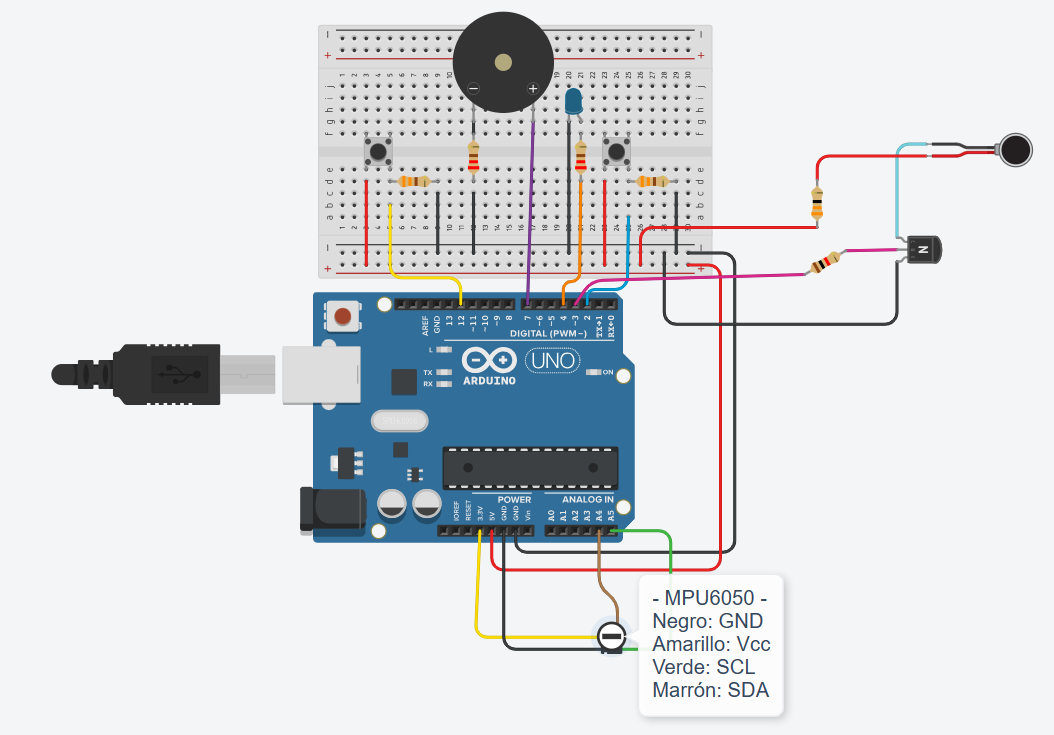
\includegraphics[width=0.8\textwidth]{img/PrototipoV2_MPU6050.png}
    \caption{Diagrama de la segunda versión del prototipo, empleando el módulo MPU-6050}
    \label{fig:ProtV2} 
\end{figure}

\begin{figure}[h]
    \centering
    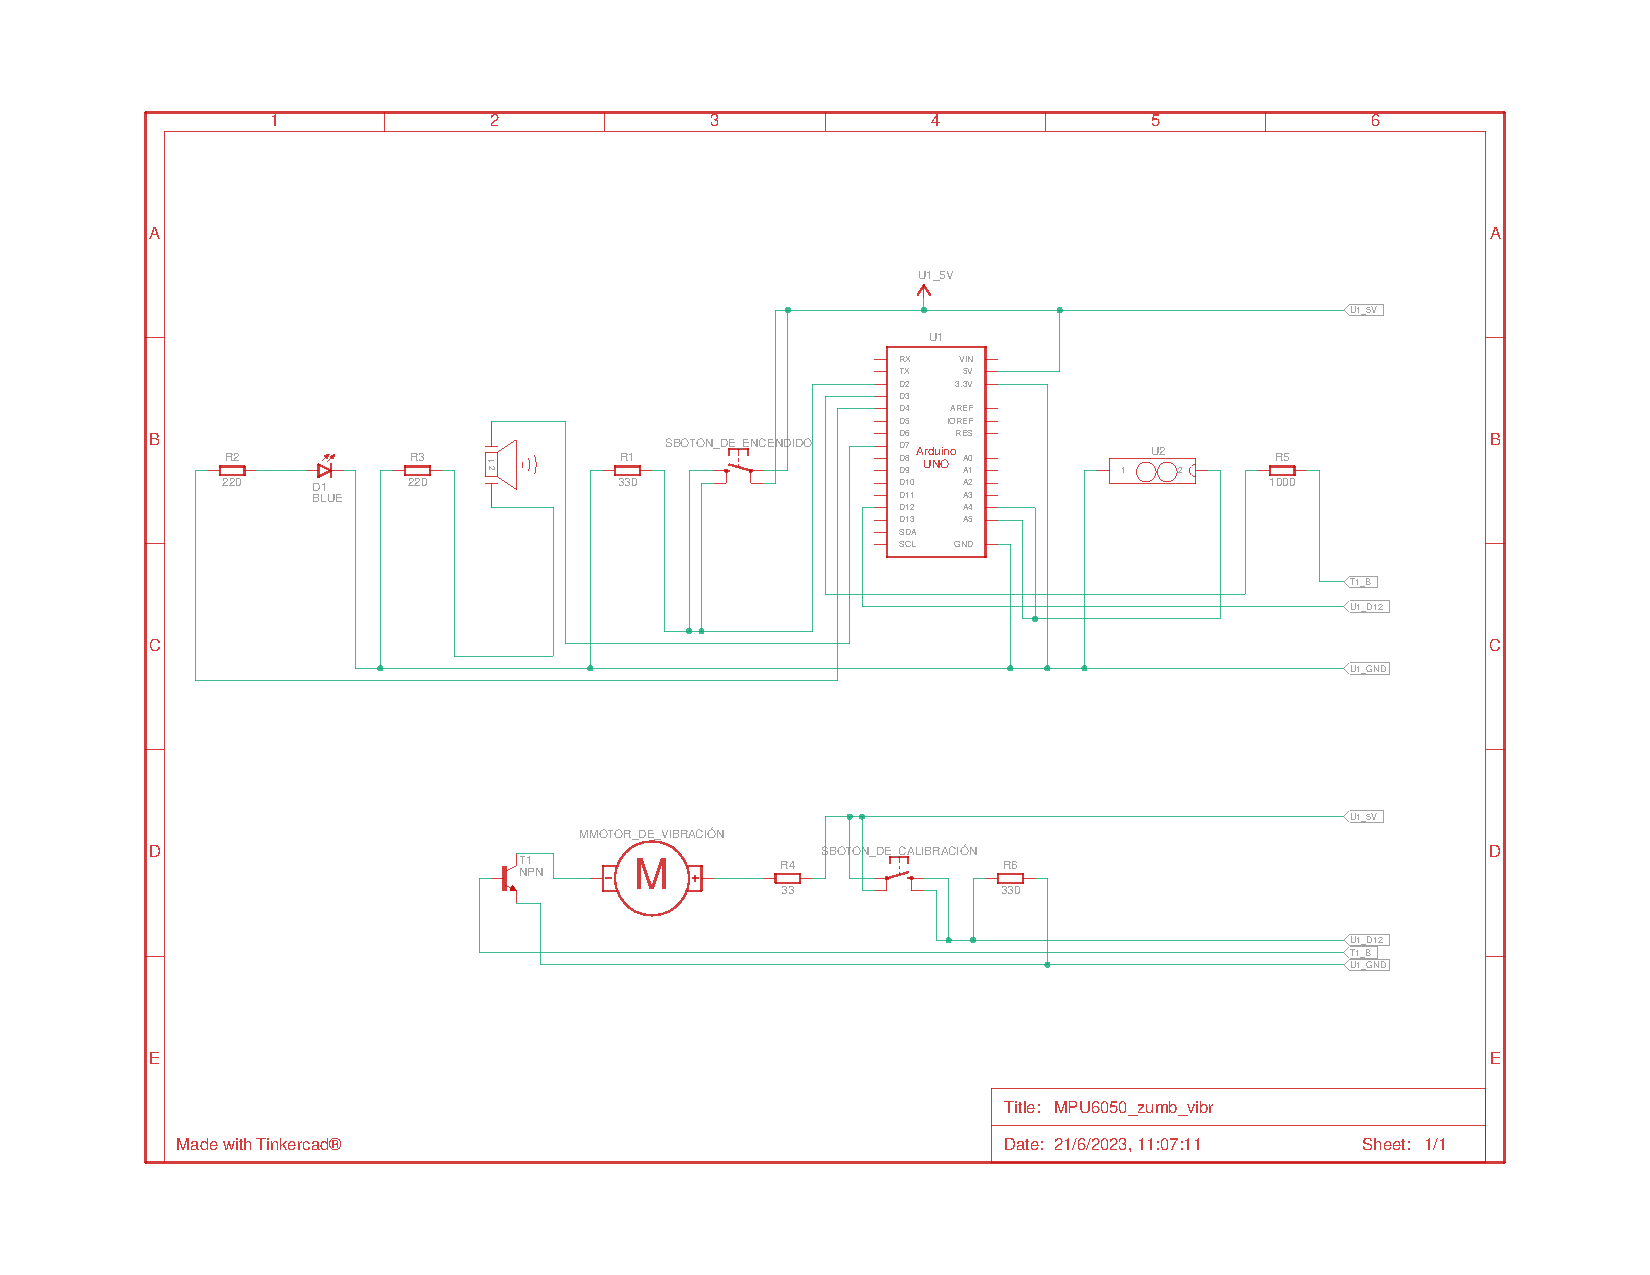
\includegraphics[width=0.9\textwidth]{img/Prot_V2_Esquema.pdf}
    \caption{Diagrama de las conexiones realizadas para la implementación de la segunda versión, siendo el módulo MPU-6050, U2.}
    \label{fig:ProtV2_esquema} 
\end{figure}


\newpage
El código empleado para el funcionamiento de esta segunda versión es el siguiente:
\begin{lstlisting}
// Led simple + Boton + Zumbador + MPU6050 + (Motor de vibracion)
// Naiara Gadea Rodriguez Gomez
// 
// Nota Si se tiene motor de vibracion descomentar las lineas de codigo correspondientes.

// Librerias I2C para controlar el sensor mpu6050 
// La libreria MPU6050.h necesita I2Cdev.h y la libreria I2Cdev.h necesita Wire.h 
#include "I2Cdev.h" 
#include "MPU6050.h" 
#include "Wire.h" 


// La direccion del MPU6050 puede ser 0x68 o 0x69, dependiendo del estado de AD0. Si no se especifica, 0x68 estara implicito.
// Se crea la variable del sensor. En este caso se esta trabajando con 0x68. Si se quiere trabajar con 0x69 hay que poner MPU6050 sensor(0x69) 
MPU6050 sensor(0x68); 

// Valores en crudo del acelerometro y giroscopio en los ejes x,y,z 
int ax, ay, az; // acelerometro 
int gx, gy, gz; // giroscopio 

float accel_ang_x, accel_ang_y, accel_ang_z; // Variables correspondientes a los angulos de inclinacion. Son los que nos interesan principalmente.

int  boton1 = 2; // Seleccion del pin del boton (pin digital)
int estado1; // Estado del boton ON/OFF
int led = 4; // Seleccion del pin del led (pin digital)
int zum = 7;// Seleccion del pin del zumbador
// int motor = 3; //Seleccion del pin del motor -Cuando se tenga el motor-
int boton2 = 12; //Boton de calibrado
int estado2;//Estado del boton de calibrado

// Otras variables
bool calibrar = false; // Variable que indica cuando seguir o no calibrando.
bool origen = true; // Para guardar los datos del primer valor tras la calibracion y comparar la diferencia de angulo de inclinacion.

// Variables usadas para filtro y promedio durante la calibracion. 
long f_ax,f_ay, f_az; 
int p_ax, p_ay, p_az; 
long f_gx,f_gy, f_gz; 
int p_gx, p_gy, p_gz; 
int counter=0;

//Valor de los offsets.
int ax_o,ay_o,az_o; 
int gx_o,gy_o,gz_o; 

float first_x, first_y, first_z; // Si no funciona correctamente desde el principio, hay que calibrar, o inicializar desde el principio.


// Variables para obtener los valores medios cada cierto tiempo.
float sum_ax, sum_ay, sum_az;
float sum_gx, sum_gy, sum_gz;
float media_ax, media_ay, media_az;
float media_gx, media_gy, media_gz;
int cont = 0;

// Angulo umbral y tiempo de aviso
int ang_aviso = 15;
int t_aviso = 5;

// Definimos las notas que se emplearan para la melodia de aviso del zumbador pasivo.
int Do = 261;
int Re = 293;
int Mi = 329;
int Fa = 349;
int Sol = 392;
int La = 440;
int Si = 493;


void setup() {
  Serial.begin(9600); // Inicializacion del monitor.
  pinMode(led, OUTPUT); // Inicializacion del pin digital led.
  pinMode(boton1, INPUT); // Inicializacion del pin digital del boton.
  pinMode(boton2,INPUT); // Inicializacion del pin boton de calibrado.
  pinMode(zum, OUTPUT); // Inicializacion del pin digital del zumbador.
  //pinMode(motor, OUTPUT);// Inicializacion del pin digital del motor de vibracion.

  Wire.begin(); // Inicializacion de la comunicacion I2C
  sensor.initialize(); // Inicializacion del sensor MPU6050

  // Al inicializar el sensor los rangos seran: 
  // Acelerometro: -2g a +2g 
  // Giroscopio: -250deg/sec a +250deg/sec 

  // Se comprueba que se ha inicializado correctamente el sensor.   
  if (sensor.testConnection()) Serial.println("Sensor iniciado correctamente"); 
  else Serial.println("Error al iniciar el sensor"); 

  // Definicion de offsets iniciales iniciales
  ax_o=sensor.getXAccelOffset(); 
  ay_o=sensor.getYAccelOffset(); 
  az_o=sensor.getZAccelOffset(); 
  gx_o=sensor.getXGyroOffset(); 
  gy_o=sensor.getYGyroOffset(); 
  gz_o=sensor.getZGyroOffset(); 
  
  Serial.println("Offsets iniciales:"); 
  Serial.print(ax_o); Serial.print("\t");  
  Serial.print(ay_o); Serial.print("\t");  
  Serial.print(az_o); Serial.print("\t");  
  Serial.print(gx_o); Serial.print("\t");  
  Serial.print(gy_o); Serial.print("\t"); 
  Serial.print(gz_o); Serial.println("\t"); 
  
  
  Serial.println("Introduce un angulo umbral(deg). "); 
  while (Serial.available()==0){
  }
  int num = Serial.parseInt();

  if (num!=0){
    Serial.println("Entra");
    ang_aviso = num;
  }
  Serial.println("Angulo umbral: "); Serial.println(ang_aviso);
  Serial.println("Introduce un tiempo de respuesta(sec). "); 
  delay(5000);
  while (Serial.available()==1){
  }

  int num2 = Serial.parseInt();

  if (num2!=0){
    t_aviso = num2;
  }
  Serial.println("Tiempo de espera para aviso: "); Serial.println(t_aviso);

}

void loop() {
  if (estado1 == LOW && digitalRead(boton1)){
    // Si se presiona el boton se ENCIENDE EL DISPOSITIVO y por lo tanto se enciende el led.
    digitalWrite(led, HIGH); // Encendido
    //delay(1000); // Durante 1 segundo (1000 ms)
    estado1 = HIGH; // Cambia el estado del boton a encendido.
    
  }
  if(estado1 == HIGH){
    // Si el dispositivo se encuentra encendido
    // Lectura de las aceleraciones y velocidades angulares y guardado en sus variables correspondientes.
    sensor.getAcceleration(&ax, &ay, &az); 
    sensor.getRotation(&gx, &gy, &gz);

    if (digitalRead(boton2) && estado2==LOW){
      // Si se presiona el boton de calibracion, cambia el estado para indicar que hay que calibrar.
      calibrar = true;
    }

    if (calibrar){
      // Si se quiere calibrar se calibra.
      calibracion();
      origen = true; // Se modifican los angulos iniciales de inclinacion.
    }else{
      
      if (cont < t_aviso/0.5){
        lecturas(); // Se realiza la lectura de los valores cada t_aviso tiempo de aviso)
        sum_ax = sum_ax + accel_ang_x;
        sum_ay = sum_ay + accel_ang_y; 
        sum_az = sum_az + accel_ang_z;

        cont++;

      } else{
        media_ax = sum_ax/(t_aviso/0.5);
        Serial.print("Valor medio de inclinacion en X: "); Serial.println(media_ax);
        media_ay = sum_ay/(t_aviso/0.5);
        Serial.print("Valor medio de inclinacion en Y: "); Serial.println(media_ay);
        media_az = sum_az/(t_aviso/0.5);
        

        // reestablecemos los sumatorios
        sum_ax = 0; 
        sum_ay = 0; 
        sum_az = 0; 
        cont = 0;

        if(abs(first_x - media_ax)<ang_aviso & abs(first_y - media_ay)<ang_aviso){// & abs(first_z - media_az)<15){
          Serial.println("Buena postura");
          noTone(zum); // NO se produce alerta
          //digitalWrite(motor, LOW);// Paramos el motor -Cuando se tenga motor.
        }else{
          Serial.println("Mala postura, ponte recto");
          //digitalWrite(motor, HIGH); //vibracion -Cuando se tenga motor.
          //delay(500);  // -Cuando se tenga motor.
          melodia(); // Se produce alerta
          
        }

      }
      if(origen){
        first_x = accel_ang_x;
        first_y = accel_ang_y;
        first_z = accel_ang_z;
        Serial.print("Valor primera medida en eje X: "); Serial.println(first_x);
        Serial.print("Valor primera medida en eje Y: "); Serial.println(first_y);
        Serial.print("Valor primera medida en eje Z: "); Serial.println(first_z);

        origen = false;
      }

    } 

    // Si se presiona el boton se apaga el dispositivo
    if (digitalRead(boton1)){
      digitalWrite(led, LOW); // Apagado
      delay(1000); // Durante 1 segundo (1000ms)
      estado1 = LOW; // Cambia el estado del boton a apagado.
    }
    
  }

}

void lecturas(){
  // Si queremos pasar las lecturas del acelerometro a m/s^2 hay que multiplicar las lecturas por (9.81/16384.0). 
  // En la componente Z se deben encontrar mediciones aproximadas a los 9.8 m/s^2 
  // Si queremos pasar las lecturas del giroscopio a deg/s (grados/s) hay que multiplicar las lecturas por (250.0/32768.0) 
  Serial.print("a[x y z]   Incl X   Incl Y  g[x y z]:\t"); 
  Serial.print(ax*(9.81/16384.0)); Serial.print("\t"); // En m/s^2
  Serial.print(ay*(9.81/16384.0)); Serial.print("\t"); // En m/s^2
  Serial.print(az*(9.81/16384.0)/2); Serial.print("\t"); // En m/s^2

  accel_ang_x=atan(ax/sqrt(pow(ay,2) + pow(az,2)))*(360.0/3.14); // En angulos de inclinacion
  Serial.print(accel_ang_x); Serial.print("\t"); 
  accel_ang_y=atan(ay/sqrt(pow(ax,2) + pow(az,2)))*(360.0/3.14); // En angulos de inclinacion
  Serial.print(accel_ang_y); Serial.print("\t"); 
  accel_ang_z=atan(az/sqrt(pow(ax,2) + pow(ay,2)))*(360.0/3.14); // En angulos de inclinacion
  Serial.print(accel_ang_z); Serial.print("\t"); 
  
  // Esto no es necesario
  Serial.print(gx*(250.0/32768.0)); Serial.print("\t"); // En grados/s
  Serial.print(gy*(250.0/32768.0)); Serial.print("\t"); // En grados/s 
  Serial.println(gz*(250.0/32768.0)); // En grados/s

  delay(500); // Mide cada 0,5 segundos. Cuando se calcule la media para comprobar que la buena postura sera cada t_aviso*2

}

void calibracion(){
  // Primero se filtran las lecturas
  f_ax = f_ax-(f_ax>>5)+ax; 
  p_ax = f_ax>>5; 

  f_ay = f_ay-(f_ay>>5)+ay; 
  p_ay = f_ay>>5; 

  f_az = f_az-(f_az>>5)+az; 
  p_az = f_az>>5; 

  f_gx = f_gx-(f_gx>>3)+gx; 
  p_gx = f_gx>>3; 

  f_gy = f_gy-(f_gy>>3)+gy; 
  p_gy = f_gy>>3; 

  f_gz = f_gz-(f_gz>>3)+gz; 
  p_gz = f_gz>>3; 
  
  // Cada 100 lecturas se corrige el offset 
  if (counter==100){ 
    // Mostramos las lecturas promedio para ver como va con la calibracion 
    Serial.print("promedio:"); Serial.print("\t"); 
    Serial.print(p_ax); Serial.print("\t"); 
    Serial.print(p_ay); Serial.print("\t"); 
    Serial.print(p_az); Serial.print("\t"); 
    Serial.print(p_gx); Serial.print("\t"); 
    Serial.print(p_gy); Serial.print("\t"); 
    Serial.println(p_gz); 
    // Basicamente se modifica constantemente el offset para que sea 0, como medida real. 
    // Se ajusta el Offset del acelerometro
    if (p_ax>0) ax_o--; 
    else {ax_o++;} 
    
    if (p_ay>0) ay_o--; 
    else {ay_o++;} 
    
    if (p_az-16384>0) az_o--; 
    else {az_o++;} 
    
    sensor.setXAccelOffset(ax_o); 
    sensor.setYAccelOffset(ay_o); 
    sensor.setZAccelOffset(az_o); 
    
    // Se ajusta el Offset del giroscopio
    if (p_gx>0) gx_o--; 
    else {gx_o++;} 
    
    if (p_gy>0) gy_o--; 
    else {gy_o++;} 
    
    if (p_gz>0) gz_o--; 
    else {gz_o++;} 

    sensor.setXGyroOffset(gx_o); 
    sensor.setYGyroOffset(gy_o); 
    sensor.setZGyroOffset(gz_o);
    
    counter=0; 

    if (p_ax>-10 & p_ax<10 & p_ay>-10 & p_ay<10 & p_az>32757 & p_az<32777 & p_gx>-10 & p_gx<10 & p_gy>-10 & p_gy<10 & p_gz>-10 & p_gz<10){
    //if (p_ax>-10 & p_ax<10 & p_ay>-10 & p_ay<10 & p_az>16374 & p_az<16394 & p_gx>-10 & p_gx<10 & p_gy>-10 & p_gy<10 & p_gz>-10 & p_gz<10){
      Serial.println("DISPOSITIVO CALIBRADO!!!");
      // El dispositivo Pita 3 veces ara indicar que se ha calibrado correctamente.
      tone(zum, Sol, 500);
      delay(200);
      noTone(zum);
      delay(200);
      tone(zum, Sol, 500);
      delay(200);
      noTone(zum);
      delay(200);
      tone(zum, Sol, 500);
      delay(200);
      noTone(zum);
      calibrar = false;
    }else{
      Serial.println("Calibrando...");
    }
  } 
  counter++;

}




void melodia(){
  // Escala de musica con el zumbador
    tone(zum, Fa, 500);
    delay(700);
    tone(zum, Sol, 500);
    delay(700);
    // Si se quiere realizar una melodia mas larga.
    //tone(zum, Sol, 500);
    //delay(700);
    //tone(zum, La, 1000);
    //delay(1700);
    //tone(zum, Sol, 500);
    //delay(700);
    //tone(zum, Fa, 500);
    //delay(700);
    //tone(zum, Sol, 500);
    //delay(700);
    //tone(zum, Do, 1000);
    //delay(1700);
    //tone(zum, Fa, 500);
    //delay(700);
    //tone(zum, La, 500);
    //delay(700);
    //tone(zum, Fa, 500);
    //delay(700);
    //tone(zum, Re, 1000);
    //delay(1700);
    
}


\end{lstlisting}

Esta versión proporciona un resultado satisfactorio, porque realiza la función del control postural correctamente, aunque hay que calibrarlo cada vez que se enciende el dispositivo y la calibración puede llevar varios minutos. Además, es posible modificar el ángulo de aviso que se quiere tener de umbral de correcta o incorrecta postura. También se puede modificar el tiempo de espera que se quiere tener para dar el aviso de una postura incorrecta, por defecto el tiempo es de 5 segundos.

Por otro lado, en esta versión se ha improbisado una base de calibración empleando material reciclado de cartón para mantener el sensor de forma plana. Además se improvisado también la forma de acoplarlo a la espalda del usuario para que se realicen mediciones correctas. Si no se coloca correctamente el sensor habría que modificar los ejes en el código, ya que no detectara de forma correcta los ángulos y esto puede ser algo complejo.


%%%%%%%%%%%%%%%%%%%%%%%%%%%%%%%%%%%%%%%
\newpage
\section{Manuales y/o Demostraciones prácticas}

\textcolor{red}{si a la vez que preparas la demostración grabas los vídeos y los incluyes puede ser bastante valorado .. además de al tribunal puedes decir que le servirá al usuario para entender como debe realizar las acciones.}

Las demostraciones prácticas se realizarán en base a una serie de pasos que se deberán realizar. Si estos pasos transcurren sin ningún contratiempo se obtendrá una ejecución exitosa. En el futuro se podrán observar y analizar los resultados.

\textcolor{red}{Se incluirá la dirección a los videos de ejemplo.}

\subsection{Demostración de la primera versión del prototipo}

En primer lugar el usuario se deberá colocar el prototipo, si es necesario puede solicitar ayuda a otra persona.

Una vez se encuentre colocado el dispositivo se encenderá presionando el botón de encendido, tras encender el prototipo se encenderá un led azul. El dispositivo empezará a controlar la postura del usuario.

\textcolor{red}{Incluir imagen del prototipo colocado y el led}

Para poder comprobar su correcto funcionamiento el usuario se inclinará hacia delante y el dispositivo al detectar un postura incorrecta dará feedback a través de sonido, y en el caso de tener añadido en el dispositivo un motor de vibración, también vibrará. Tras unos segundos el usuario volverá a una posición correcta, al corregir su postura el dispositivo dejará de sonar y de vibrar.

\textcolor{red}{Incluir imagen de postura correcta y de postura incorrecta}

Se volverá a comprobar que funciona correctamente haciendo que el usuario se vuelva a inclinar hacia delante, el dispositivo volverá a indicar que se ha establecido una mala postura y el usuario gracias al aviso sabrá que deberá corregir su postura, una vez el usuario haya corregido su postura el dispositivo dejará de pitar.

Se realizarán pruebas en las que el usuario se agache o salte o ande para ver cuando da problemas este dispositivo, debido a su sensibilidad a vibraciones. Los problemas detectados son aquellos que se intentarán solucionar en la segunda version donde se empleará un sensor más complejo.

Por último, el dispositivo se apagará empleando el botón de encendido/ apagado.


\subsection{Demostración de la primera versión del prototipo}

Para la demostración de esta segunda versión en la que se emplea un sensor más complejo y preciso, el sensor MPU6050\cite{MPU6050_1,MPU6050_2}, el primer paso es que el usuario se coloque el prototipo.

\textcolor{red}{Imagen del dispositivo colocado}

Una vez el dispositivo se encuentre correctamente colocado el sistema pedirá el ángulo de aviso y el tiempo de aviso, si el usuario no indica estos datos se toma como valor por defecto 15º y 5 segundos. Se debe encender el dispositivo presionando el botón de encendido. Al encender el prototipo se encenderá un led de color azul y el dispositivo comenzará a controlar la postura. Si es la primera vez que se conecta al portatil el dispositivo deberá calibrar el dispositivo. En ese momento el usuario deberá presionar el botón de calibración para calibrar el dispositivo. Durante la calibración el dispositivo no debe moverse y puede tardar varios minutos. Una vez calibrado, el dispositivo pitará 3 veces o vibrará tres veces.

\textcolor{red}{Incluir imagen de la pantalla cuando el sistema solicita el ángulo y el tiempo}

\textcolor{red}{Incluir imagen del dispositivo calibrando.}


Tras la calibración el prototipo comenzará el control postural de forma correcta.

Para comprobar su funcionamiento la persona se inclinará ligeramente hacia delante, si supera el umbral, en este caso 15º, el dispositivo pitará y vibrará a modo de feedback. La persona gracias al biofeedback corregirá su postura, una vez adoptada una postura correcta el dispositivo dejará de emitir sonido y vibración. Se volverá a realizar una medición de prueba pero está vez el usuario se encontrará andando.

\textcolor{red}{Incluir imagen del dispositivo colocado y de la persona en postura correcta e incorrecta}

\textcolor{red}{Incluir pantallazo del sistema cuando indica una postura correcta y otra incorrecta}

El usuario se inclinará de nuevo ligeramente y el dispositivo indicará una mala postura, la persona corregirá su postura tras conocer su estado gracias al dispositivo, y una vez corregida la postura el dispositivo dejará de emitir la alerta.

Se puede probar la mayor precisión de esta versión realizando los movimientos que perturbaban en la versión anterior, como agacharse o saltar donde el sensor deberá no deberá emitir alerta.

Queda comprobado que con esta versión se obtiene un dispositivo más preciso y personalizado y, además, se puede emplear tanto para uso en personas sentadas o en movimiento (andando).

Por último, se deberá apagar el dispositivo con el botón de encendido/apagado una vez ya no se requiera el control postural.

